% Example from below
% https://www.overleaf.com/learn/latex/Learn_LaTeX_in_30_minutes
\documentclass[12pt, A4]{article} %  defines the overall class (type) of document.
%if we use book class instead of article, we can use \chapter{Let's begin} before  \section{•}
\usepackage{graphicx} %LaTeX package to import graphics
%\usepackage[bottom=0.5cm, right=1.5cm, left=1.5cm, top=1.5cm]{geometry} % to change the margin of Page
\graphicspath{{images/}} %configuring the graphicx package
 \usepackage{hyperref}


% ///////Below is components for title page ///////////
\title{A Beginner's Guide to  Beijing DWIN Technology LCD 

Demo on DMT10768T150\_ 18WT}
\author{Sannan Ahmed, Ali Harman}
\date{\today} %\date{August 2022}
%/////////////////////////////


% any thing above \begin is called preamble

\begin{document}

%if you press two "enter" key then new paragraph will created

% ///////this is to make a title page///////////
\begin{titlepage}
\maketitle
\thispagestyle{empty} %this will clear the number from the title page
\end{titlepage}
%////////////////////////////////

%to add a table of contents (table of contents need to be updated (cut then Quick Build & paste then Quick Build) if any content changes.


\section{Preparing a SD card}

We have used 32GB SD card for development. we first make a partition then make a 4GB volume using disk management.Then we format the card using fat32 file system and we will make 4kb sectors, as shown in the figure below.\\


\begin{figure}[!htb] %[!htb] is used to place image where it is in editor
	\centering
	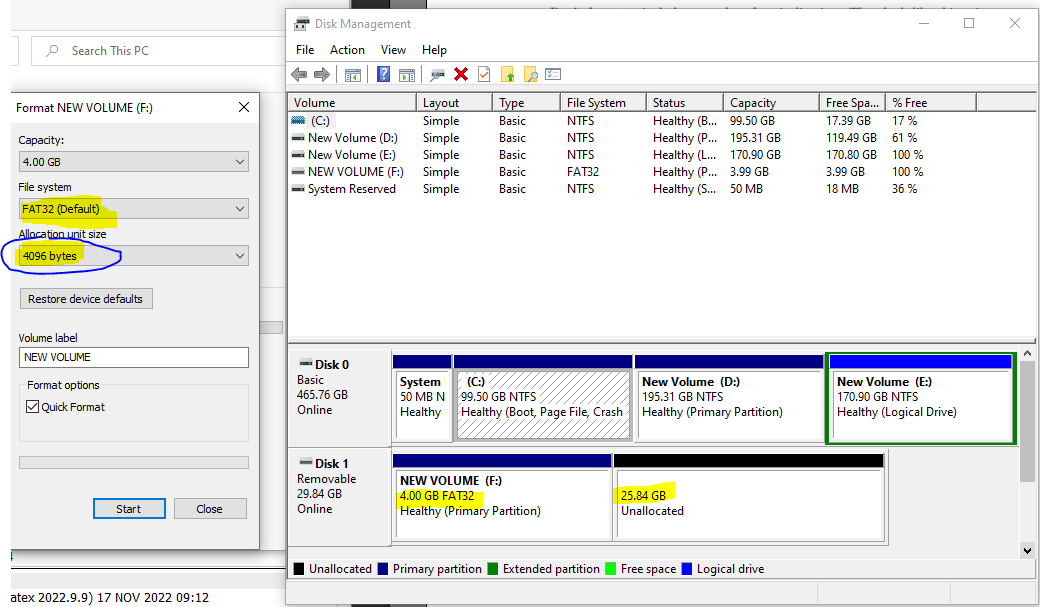
\includegraphics[width=15cm]{sdCard} 
	\caption{SD card formatting procedure.\\}
\end{figure}


\emph{\textit{Note: For 16GB card we dont have to make 4GB volume. We can directly make 4kb sector in format}}

%this is how to go on new page
\newpage


\section{How to insert image in DGUS}

First open the software (DGUS\_V5.08.exe) then make a new project (or open existing one), then inset the image using the plus sign at the left of the software interface. Then press "Save" button, then press "Generate" button (these button are present on the home tab of the top bar)

\emph{\textit{Note: We recommend that image should be in bmp format. since we are facing some issues in 16bit so we are making images in 24bit format (windows)}}

\begin{figure}[!htb] %[!htb] is used to place image where it is in editor
	\centering
	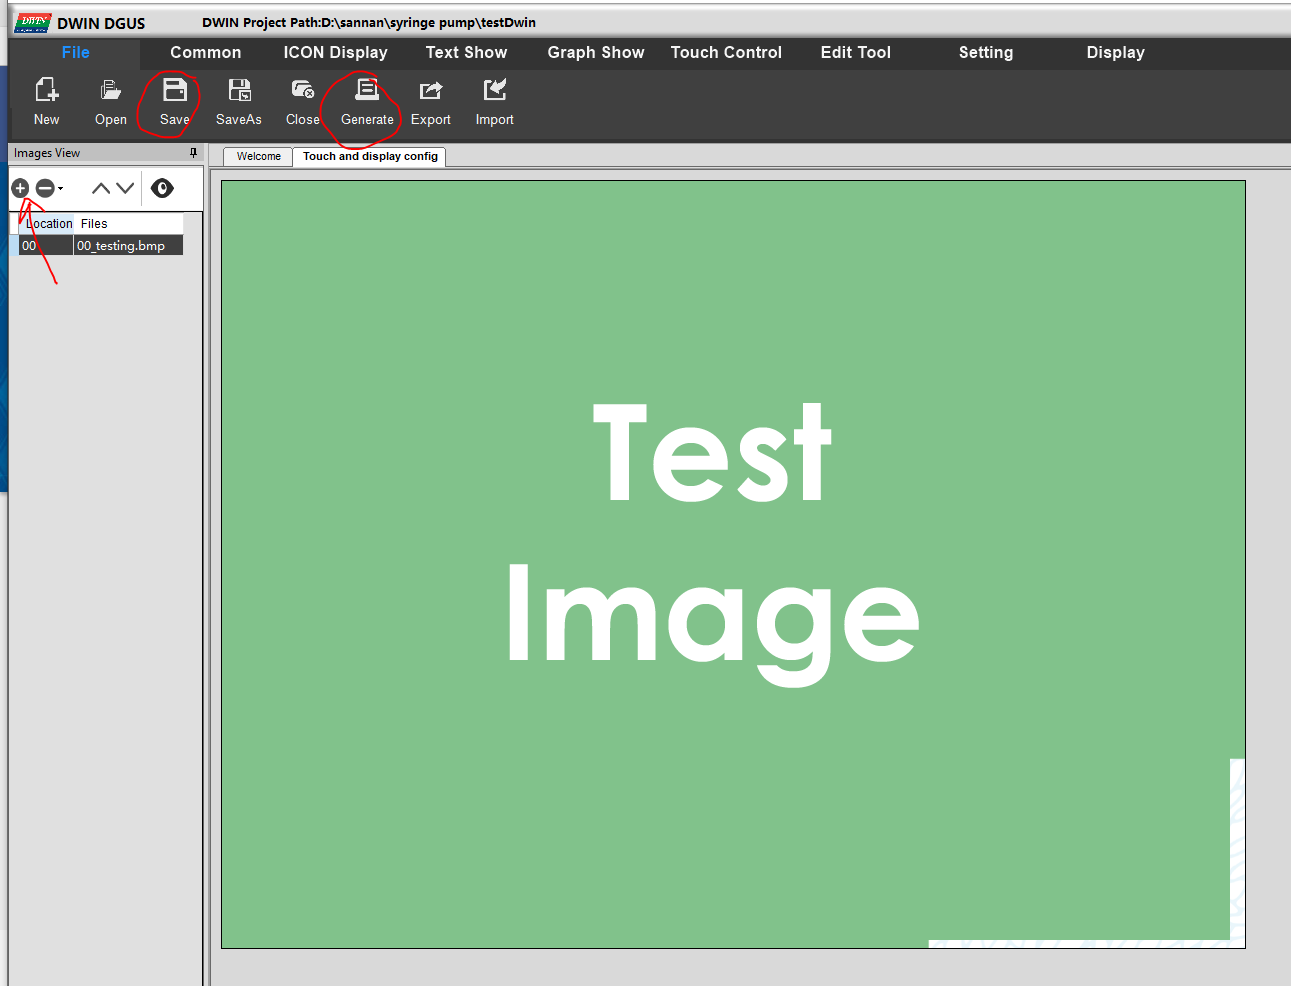
\includegraphics[width=15cm]{imageInsert} 
	\caption{Insert background image.\\}
\end{figure}

\newpage

\section{How to insert image animation in DGUS}

for image animation to work the image should be in bmp and of 24bit. insert the image animation from the top bar. and select the start and end image as shown in the figure below.

\begin{figure}[!htb] %[!htb] is used to place image where it is in editor
	\centering
	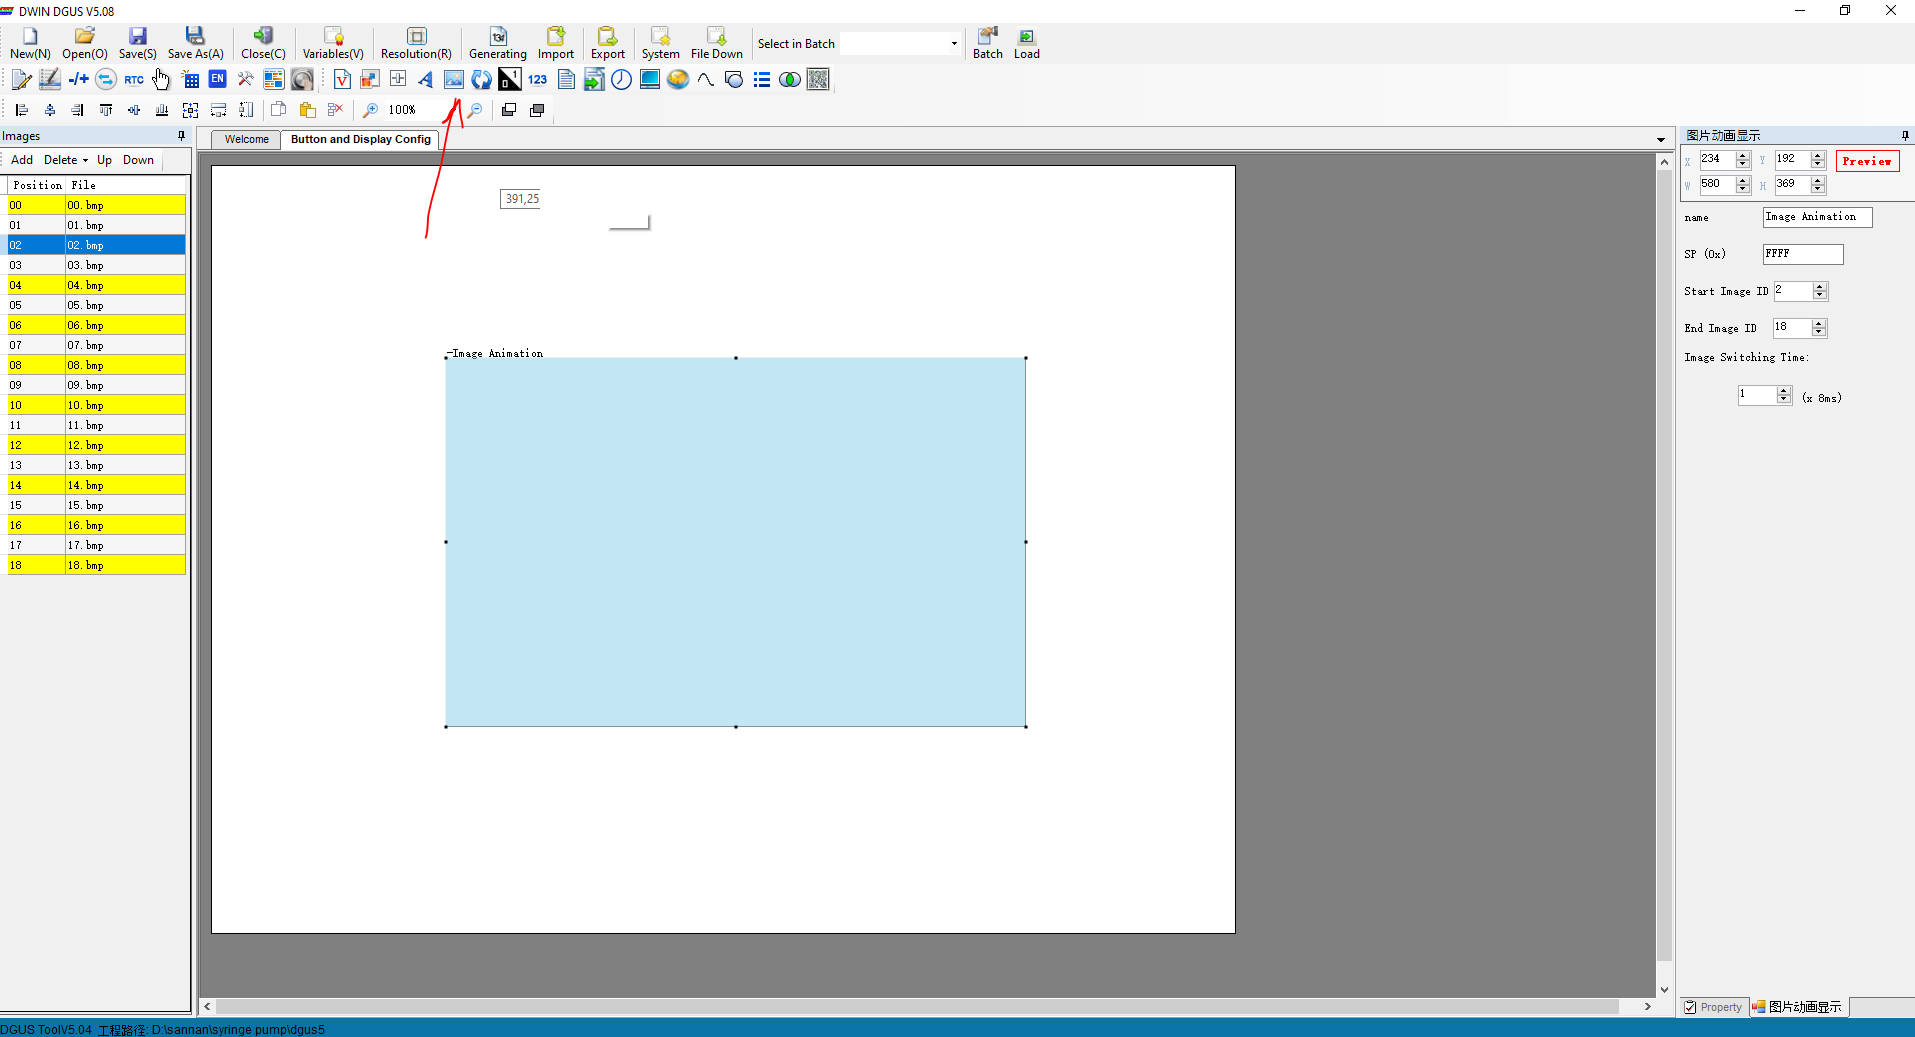
\includegraphics[width=15cm]{imageAnimation} 
	\caption{Insert image animation.\\ \\}
\end{figure}

\emph{\textit{Note: For Converting the image from png to BMP of 24bit we can use the following python script (Adjust numbering in python script as needed)}}

\href{https://colab.research.google.com/drive/1hgpBBuKO39BK6Y1HG6px_PaGPOhLLVv5?usp=sharing}{ \\  \textbf{ \centerline{Link for python script} }}


\textit{(But we need to change the name of the images in the output folder)}
\newpage


\section{How to insert Basic touch control in DGUS}

insert basic touch control from the top bar. in button effect, select the map image (touch color image). In jump to, select the page where you want to jump. 

\begin{figure}[!htb] %[!htb] is used to place image where it is in editor
	\centering
	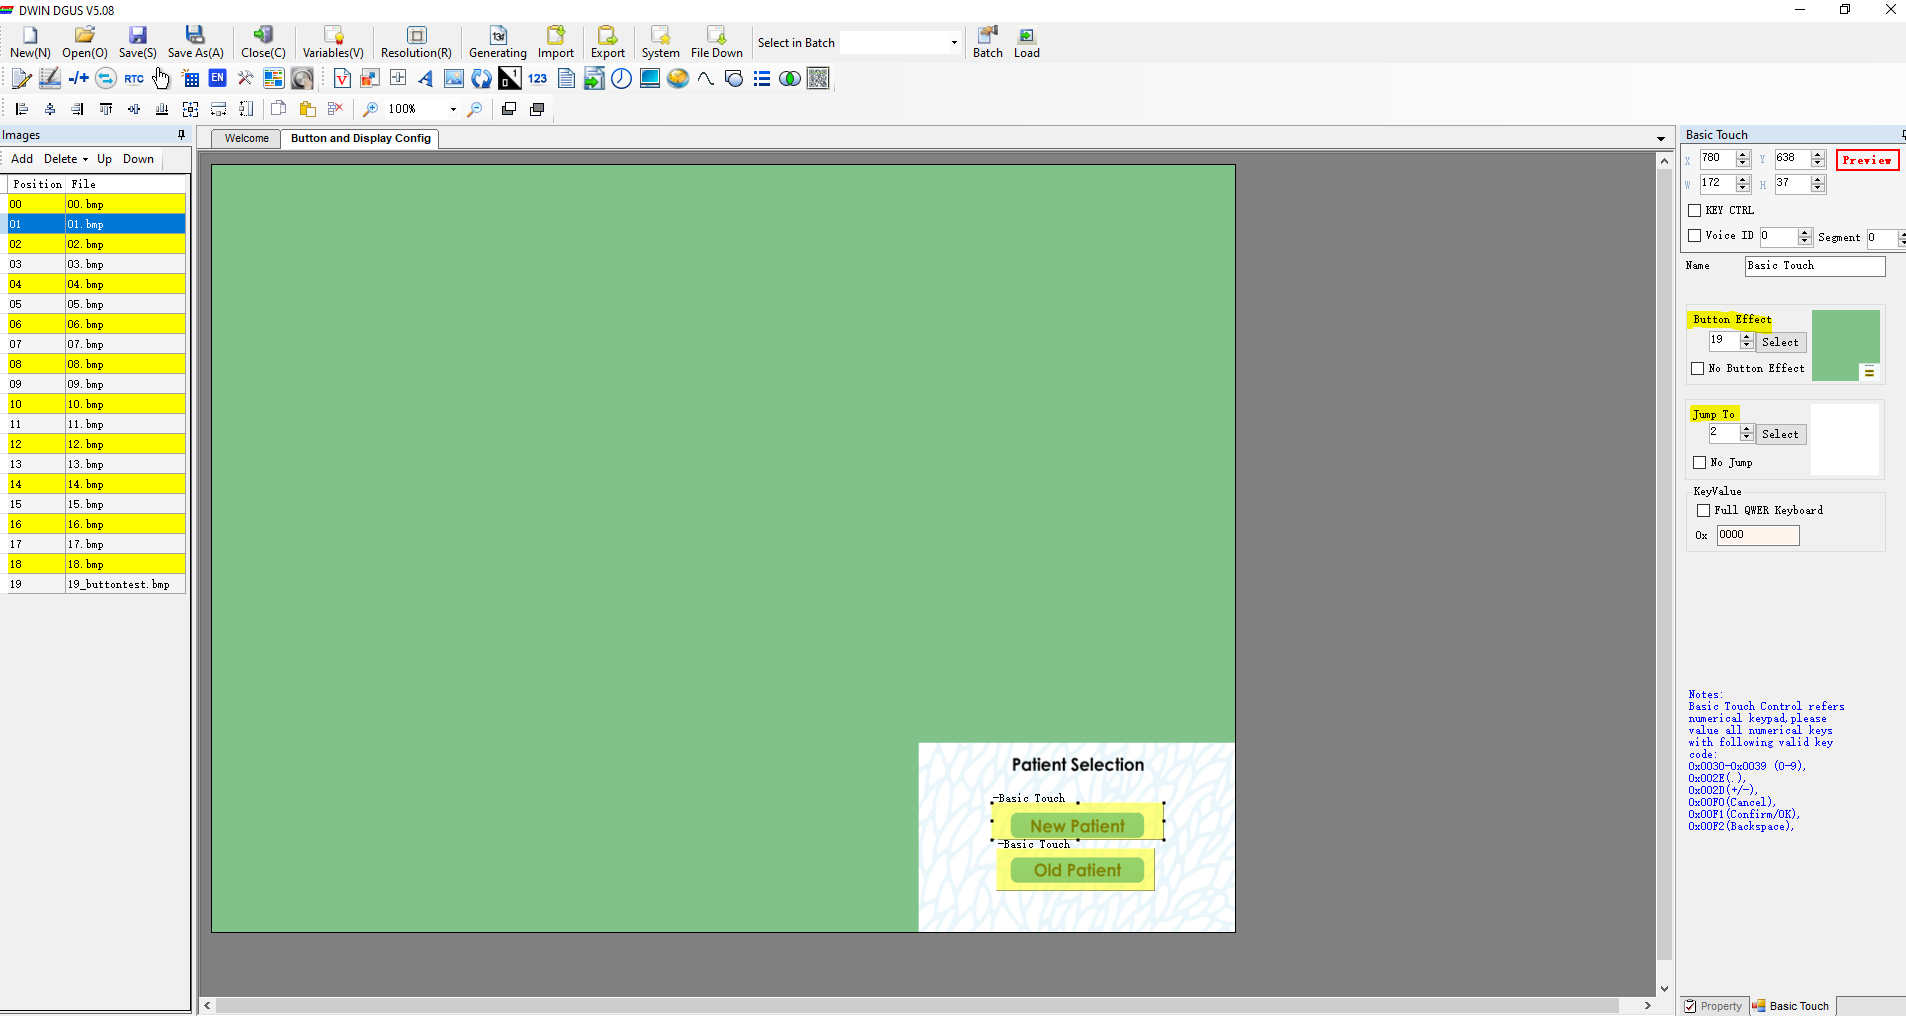
\includegraphics[width=15cm]{basicTouch} 
	\caption{Insert basic touch button.\\ \\}
\end{figure}

\emph{For basic touch control, we have to made two images. One for foreground and other for background. }

\newpage

\section{How to insert Data Variable and Return key code in DGUS}
insert data variable from the top bar. in data variable, set the vp address (variable address), text color, var type etc. 

\begin{figure}[!htb] %[!htb] is used to place image where it is in editor
	\centering
	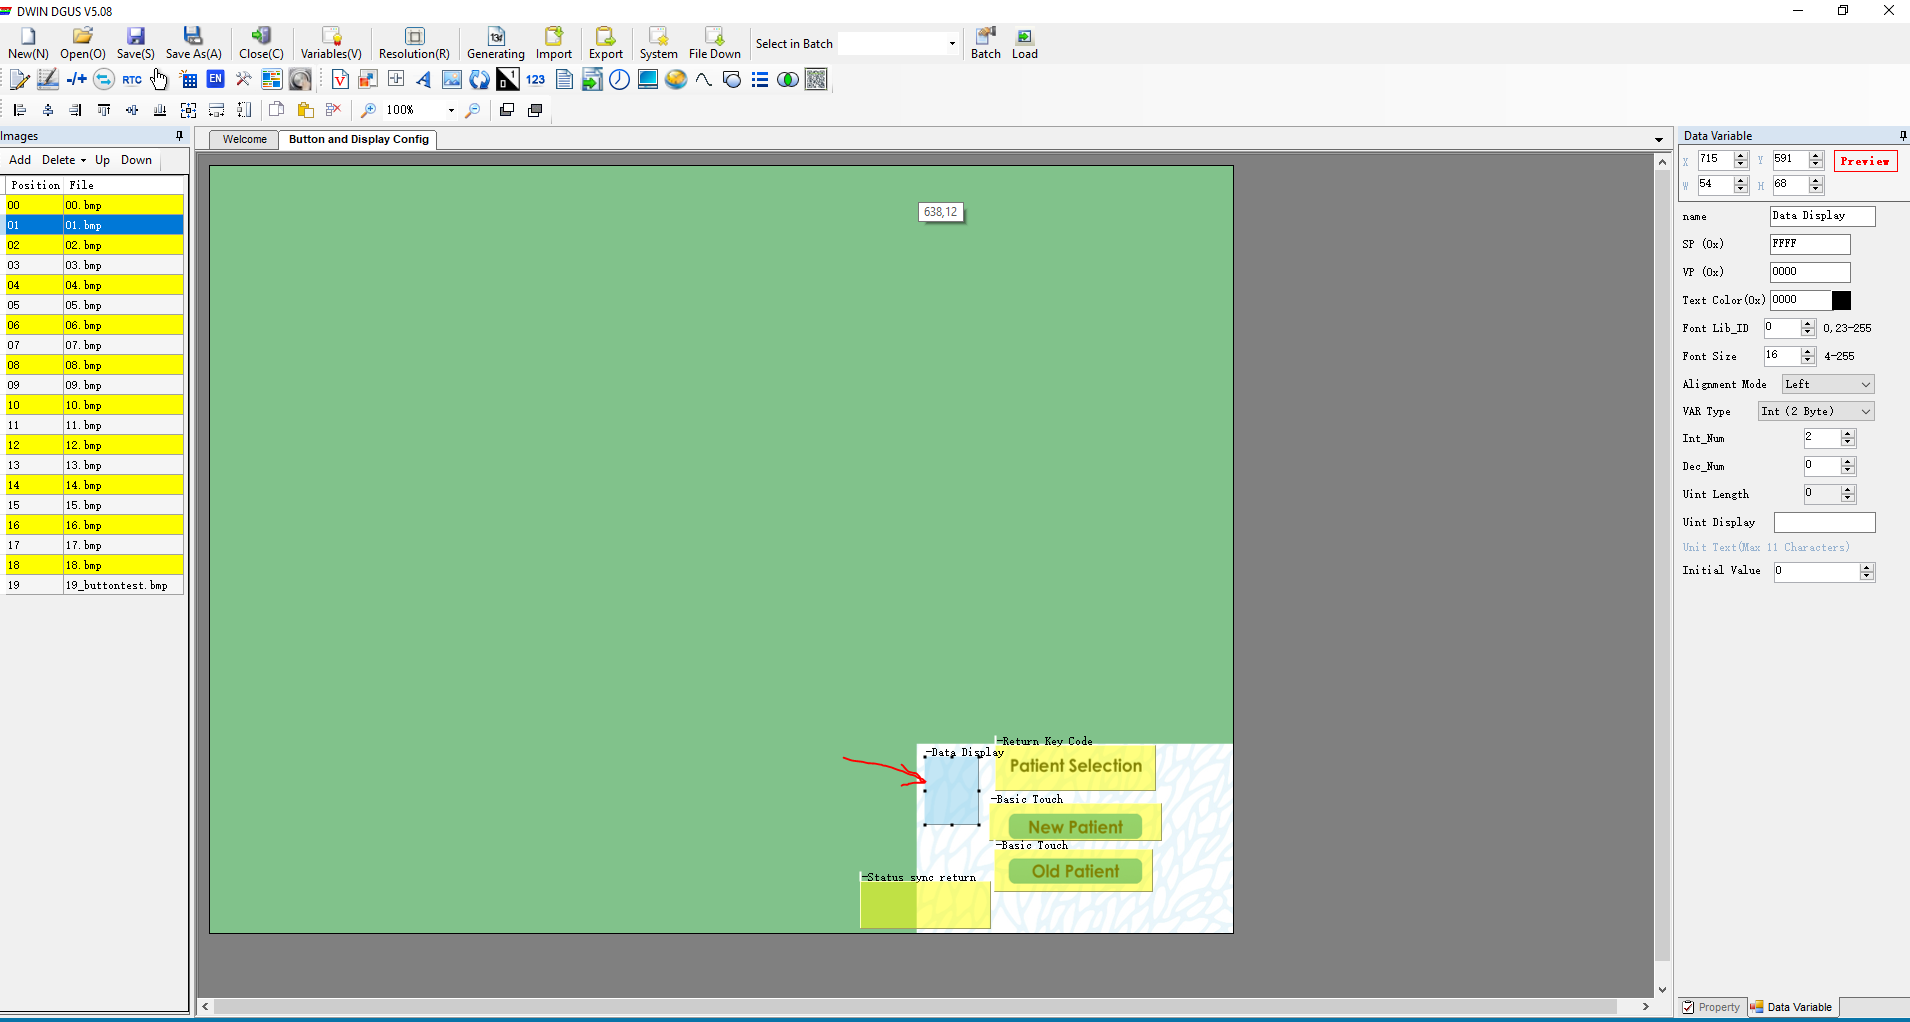
\includegraphics[width=11cm]{dataDisplay} 
	\caption{Insert data display.\\}
\end{figure}
We can use "Return key code" to set the value in the Data variable. we van also use button effect and jump to.\\
\begin{figure}[!htb] %[!htb] is used to place image where it is in editor
	\centering
	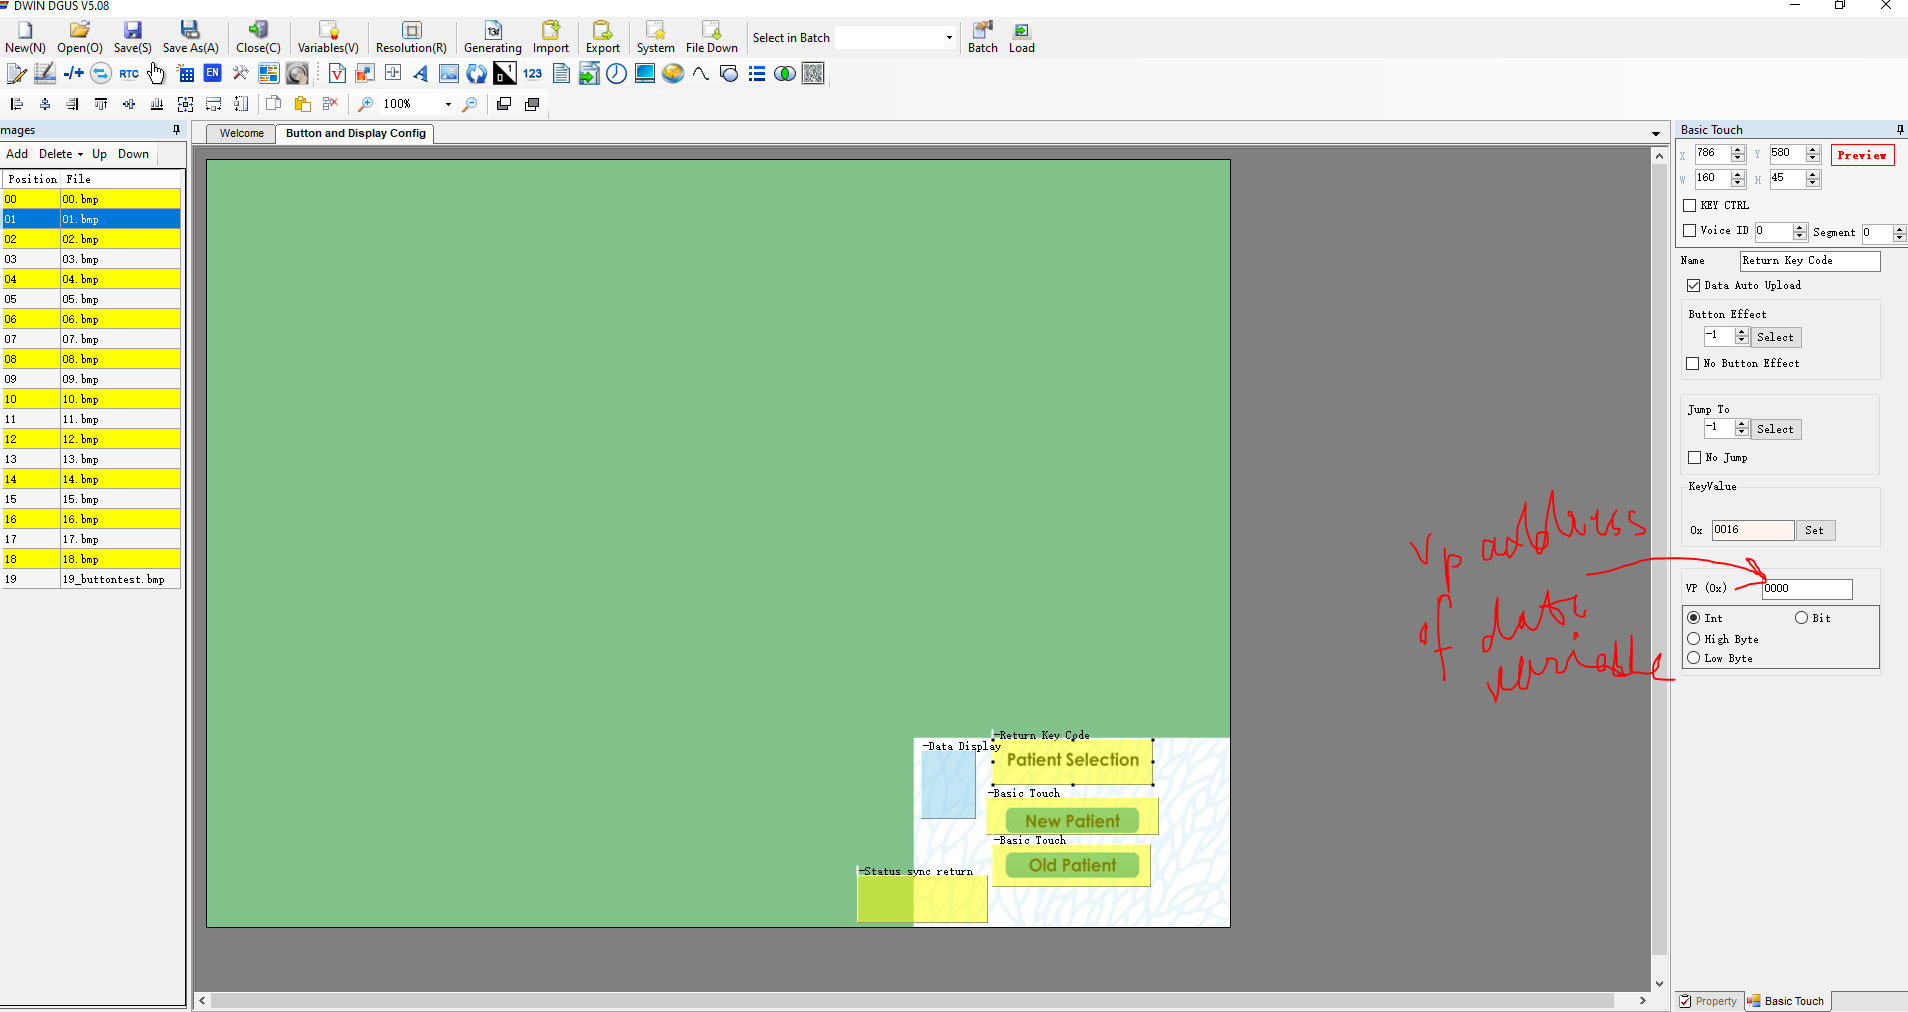
\includegraphics[width=11cm]{returnKeyCode} 
	\caption{Insert return key code.\\}
\end{figure}

\newpage

\section{How to change system configuration in DGUS}
system configuration can be changed from the DGUS software or by changing the config file. as follows.
\begin{figure}[!htb] %[!htb] is used to place image where it is in editor
	\centering
	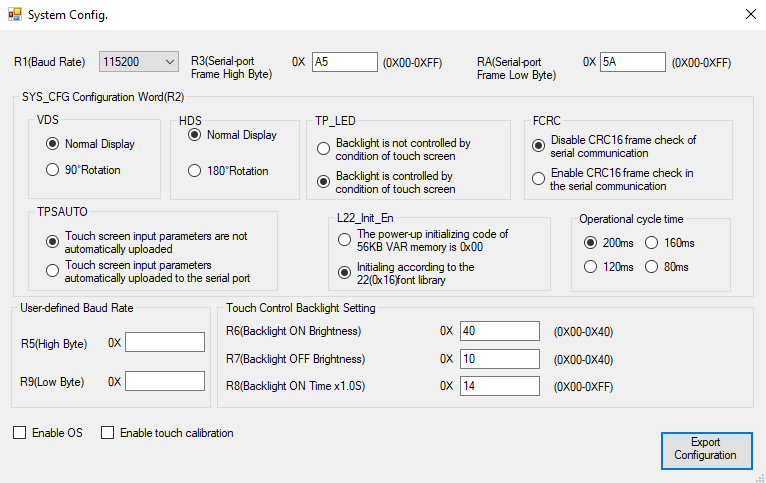
\includegraphics[width=12cm]{systemConfig} 
	\caption{system configuration.\\}
\end{figure}

\begin{figure}[!htb] %[!htb] is used to place image where it is in editor
	\centering
	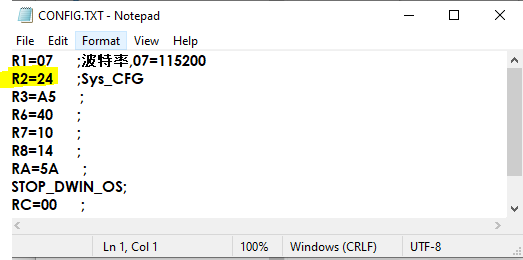
\includegraphics[width=10cm]{configFile} 
	\caption{config text file in dwin folder.\\}
\end{figure}
\newpage

\section{How to Receive \& Send data Serially in DGUS}

We can send data to MCU using "Status sync return", which Return different data to the VP/UART/Register during Press, Continuous press, Loosen press. 

Return Mode: 0x00 means no data return;
\begin{itemize}
\item 0x01 means return the data to the VP
\item 0x02 means return the data to the UART
\item 0x03 means return the data to the Register/System Variables interface
\end{itemize}
                         
For T5L series, only have 0x01 mode, but could support VP, UART, Register/ System Variables interface together\\

 
\emph{Note: If LCD supports RS485 then use Max485 to convert data to Rx or Tx.}
\begin{figure}[!htb] %[!htb] is used to place image where it is in editor
	\centering
	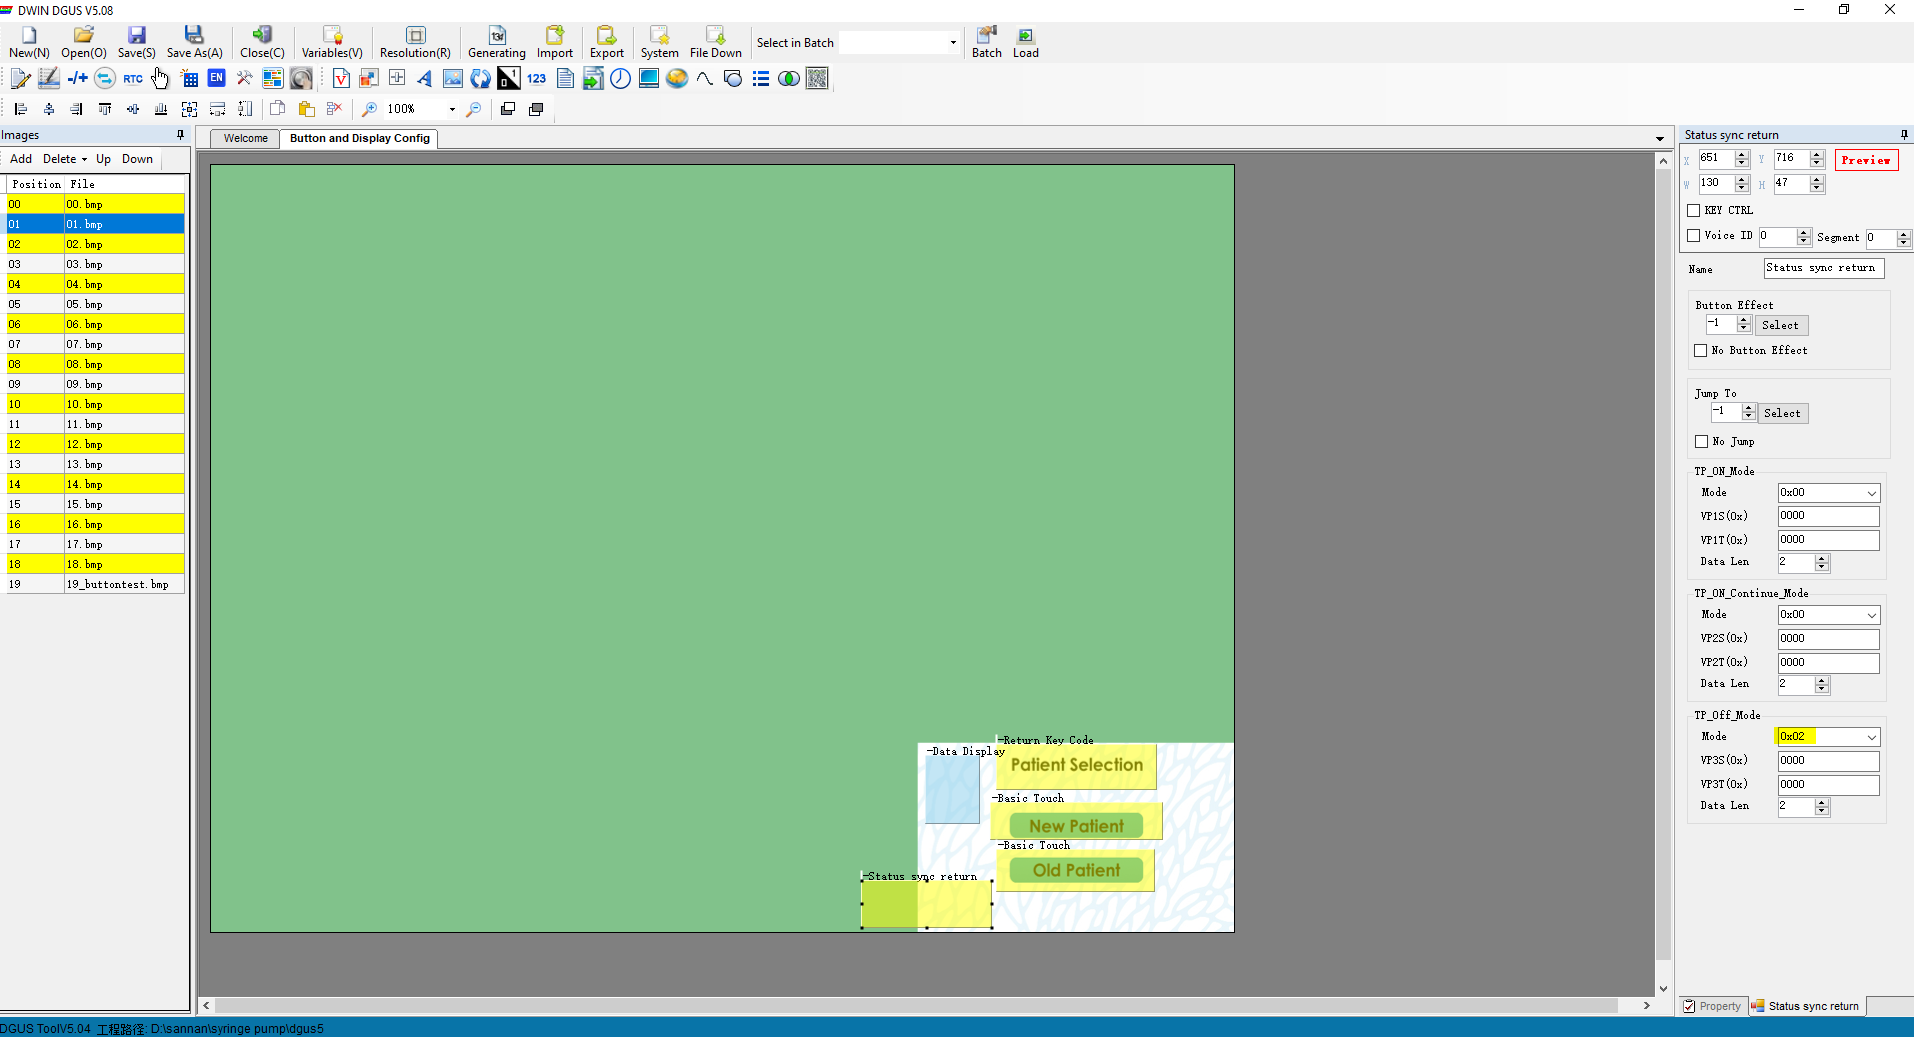
\includegraphics[width=15cm]{statusSync} 
	\caption{Status Sync Return.\\}
\end{figure}

We can use "Return key code" to set the value in the Data variable. we van also use button effect and jump to.\\

For data to send serially insert the configuration file "CONFIG.TXT" in the DWIN\_SET folder.\\ \\
Paste the following in the CONFIG.TXT file\\ \\
R1=07 ; Baud rate, 0x07: 115200bps.\\
R2=20 ; SYS\_CFG, enable sleep mode if no operation.\\
R6=40 ; Brightness of backlight, 0x40: 100\% brightness.\\
R7=10 ; Brightness of backlight of sleep mode, 0x10: 25\% brightness.\\
R8=14 ; Light-up time,units: 1.0 seconds,0x14=20 seconds.\\
R3=A5 ; High-byte of frame header: 0xA5.\\
RA=5A ; Low-byte of frame header: 0x5A.\\
STOP\_DWIN\_OS; \\

\begin{figure}[!htb] %[!htb] is used to place image where it is in editor
	\centering
	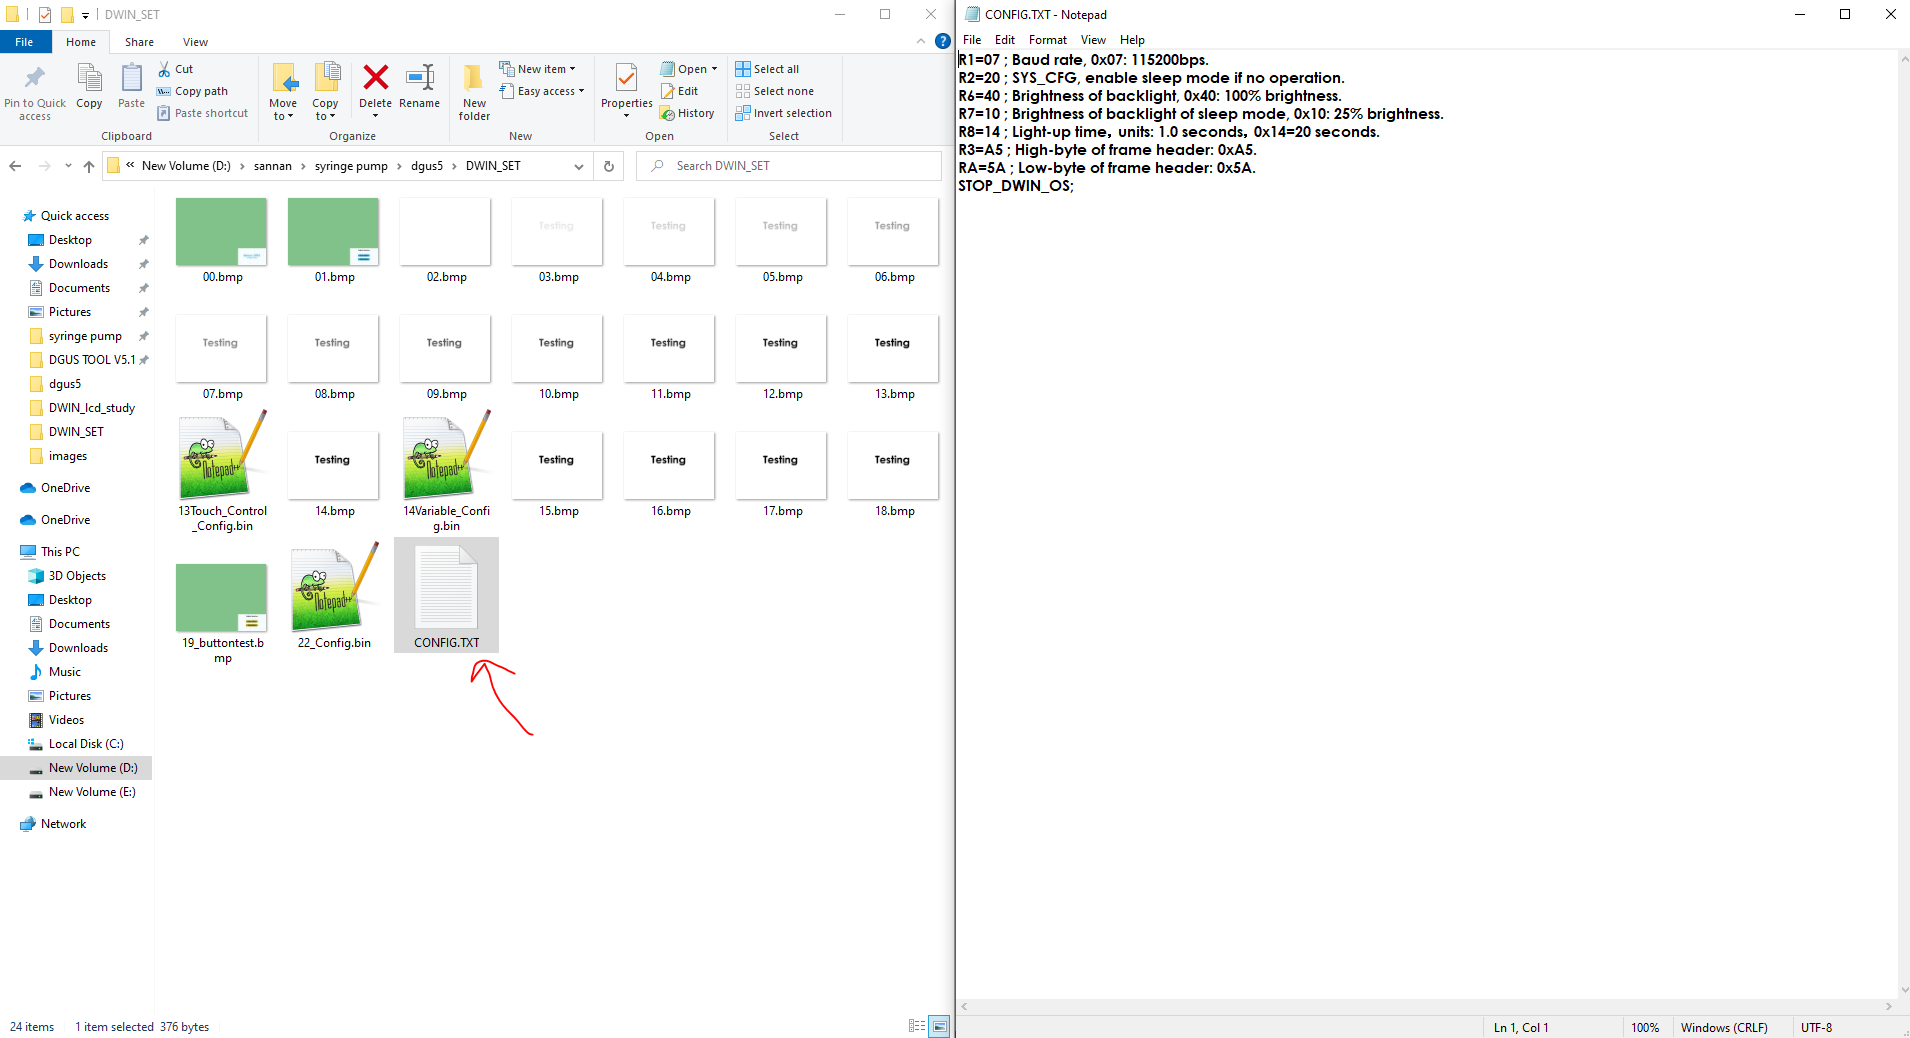
\includegraphics[width=15cm]{config} 
	\caption{CONFIG file in DWIN\_SET folder.\\}
\end{figure}

\newpage

For sending the data to LCD (DGUS) we use the following command.\\

{\huge 0xa55a058200000010\\}


We can send the command using termite.\\ 
\emph{Note: Following setting need to be done in termite for sending the data. we send the data as shown in the figure.}

\begin{center}
\begin{tabular}{ c c }
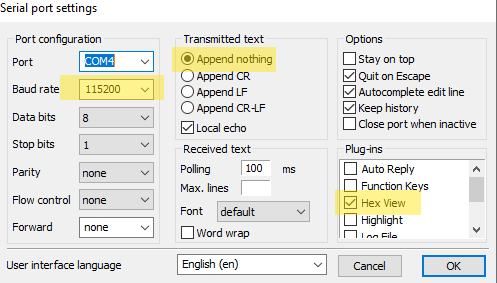
\includegraphics[width=9cm , height=7cm]{termite} & \includegraphics[width=6cm , height=7cm]{termiteWindow}
    \end{tabular}
\end{center}
\begin{figure}[!htb] %[!htb] is used to place image where it is in editor
	\centering
	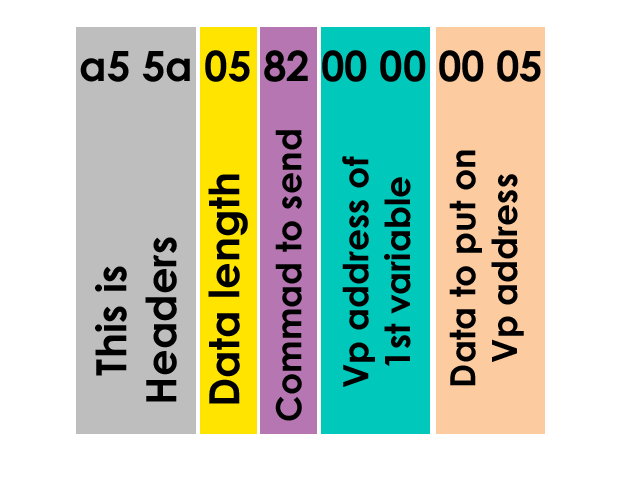
\includegraphics[width=7cm]{sendCommand} 
	\caption{Send command to LCD\\}
\end{figure}

\newpage

\section{How to insert keyboard in DGUS}
Insert text display, where you want to show the text. Also insert text input on top of the text display. insert following settings.

\begin{itemize}
\item Data Auto Upload
\item Insert the vp address (vp address of text input should be same as the text display)
\item input mode: Re-open
\item text lenght: 10
\item Click Keyboard Settings. (to select the keyboard image)
\item clipping rectangle will be used to crop the keyboard.
\item paste location can be same as first coordinate.
\item in the keyboard diagram, make basic touch for buttons.
\end{itemize}

"Text input" parameters is shown in the below figure.

\begin{figure}[!htb] %[!htb] is used to place image where it is in editor
	\centering
	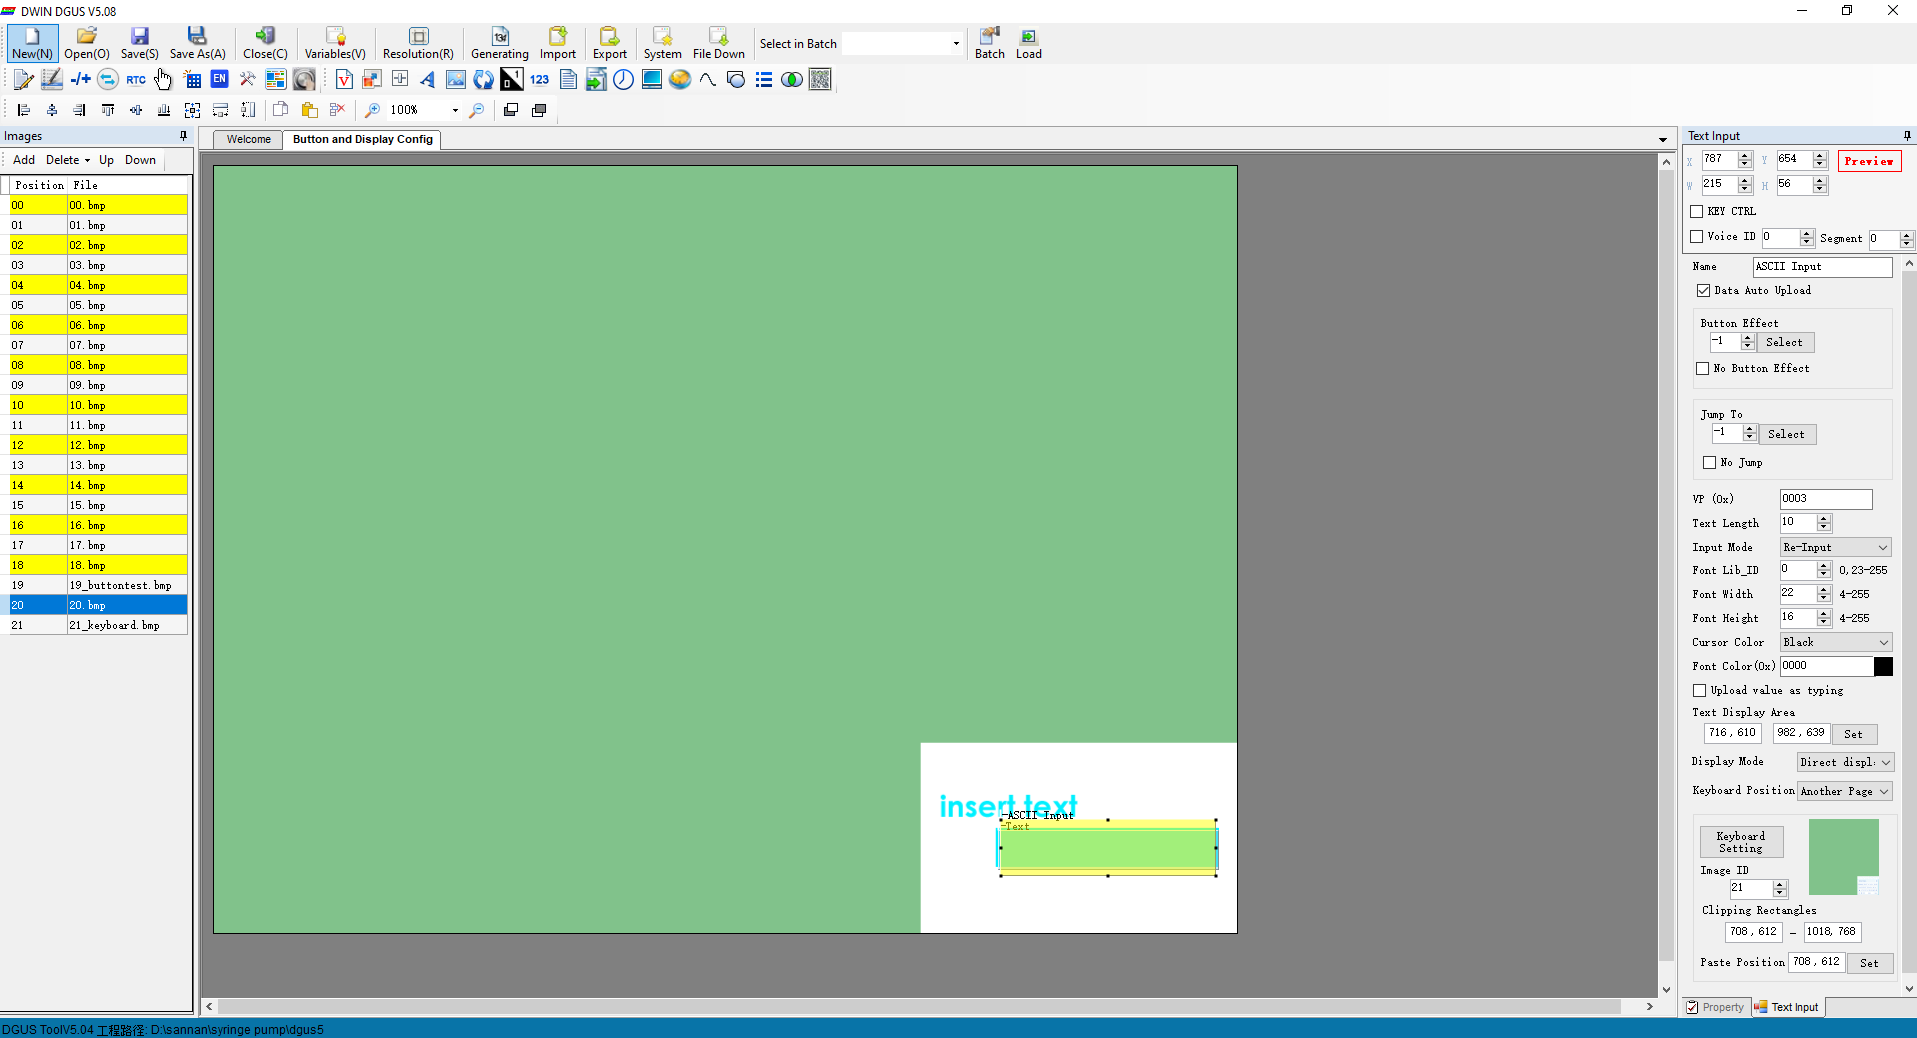
\includegraphics[width=11cm]{textInput} 
	\caption{Text Input parameters.\\}
\end{figure}

\newpage


\section{How to use fonts in DGUS}
The Dwin lcd have 3 types of fonts, which are:
\begin{itemize}
\item Zero font ( .HZK)
\item Gray font (.Bin)
\item Unicode/ASCII ( .DZK)
\end{itemize}
The TL5 Lcd support \textbf{Zero font} and \textbf{Unicode/ASCII} only, where as the TL7 seriese of Lcd support all three type of fonts.
\begin{figure}[!htb] %[!htb] is used to place image where it is in editor
	\centering
	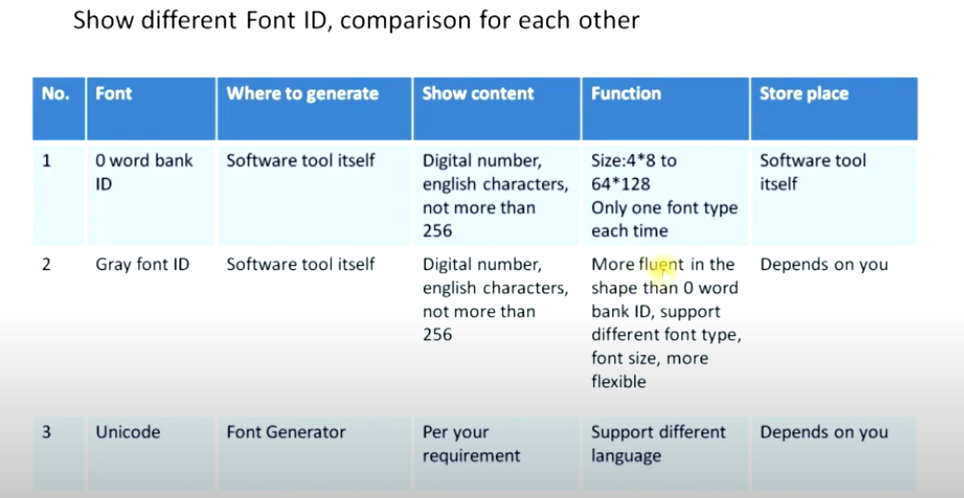
\includegraphics[width=12cm]{fontType} 
	\caption{Font generation types.\\}
\end{figure}
\subsection{Zero Font}
The 'Zero Font' or '0 word bank ID' is the font that is stored at '0' location in the lcd flash, it is the default font that the lcd will use.Only \emph{one zero font} can be created, more fonts are created using other methods.

In the welcome page of DGUS software (DGUS V5.08), Click "No. 0 font lab" button. to open the software that creates fonts, or run the applicatin PATH "DGUS TOOL V5.10/DW0\_Font" to lanch it.

Select the font type from 'Font Selection' and adjust the different \emph{scale} and \emph{shift} till later are not cliping,(tip: Use a monospace font, it will provide equal spacing, if using manual spacing in setting). Press the "Create" button and the software will start creating the font, after finish the font will be created in "DGUS TOOL V5.10" folder, copy it to your project "DWIN\_Set" Folder.
\begin{figure}[!htb] %[!htb] is used to place image where it is in editor
	\centering
	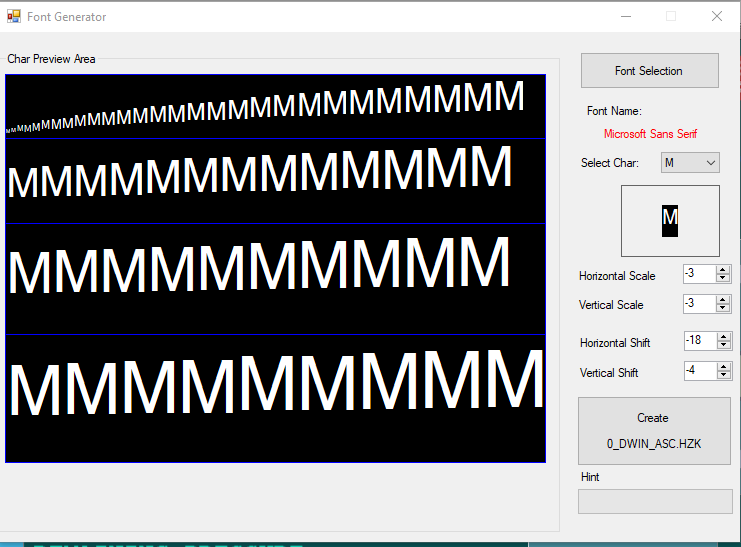
\includegraphics[width=12cm]{zero-font} 
	\caption{Zero Font generator.\\}
\end{figure}
The setting used for Zero font are shown in the figure.
\begin{figure}[!htb] %[!htb] is used to place image where it is in editor
	\centering
	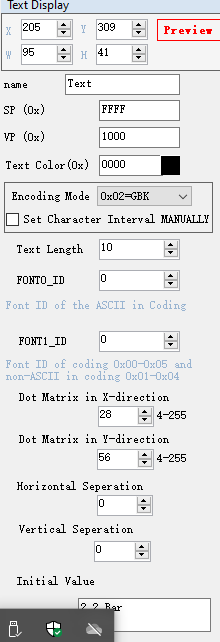
\includegraphics[width=5cm]{zero-font-config}
	\caption{Setting for usnig zero font in editorr.\\}
\end{figure}
Font ID is '0' for both ASCII and non-ASCII for 'zero font'. Uncheck 'set character interval manually' so that spacing is adjusted automatically (usefull for non-monospace fonts). In 'zero font' \emph{Dot Matrix in X-direction} and \emph{Dot Matrix in Y-direction} can have any value, Y-direction is two times X-direction. In other font type we will see that this is not the case.
\newpage

\section{How to change page in DGUS}
In order to change the page in dmt10768t150\_18wt (obselete). We to send the following command to change the value of the register (0x03).\\

{\huge 0xa55a0480030002\\}

\begin{figure}[!htb] %[!htb] is used to place image where it is in editor
	\centering
	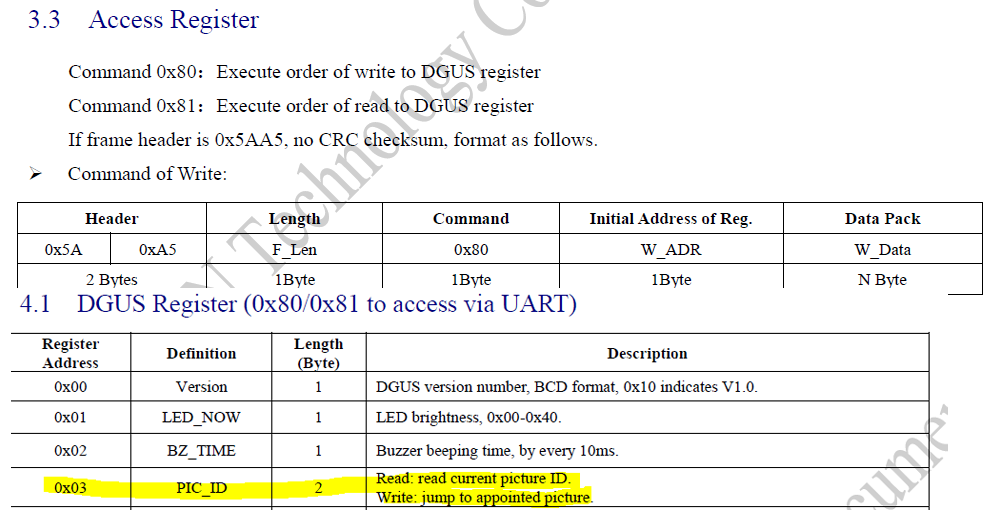
\includegraphics[width=12cm]{pageChange} 
	\caption{page Change.\\}
\end{figure}
\end{document}